\chapter{Appendix}
\section{Missing Data Mechanisms}
\label{app:apdx}
There are three mechanisms of missing data. It is important to understand what type of missing data we have so that we can use methods that are suited for that type. 
Before we begin, we will need some notation. It is not constant throughout the literature, so I caution you to look at the author's notation before reading any other literature. I will give the symbols I will be using along with words to describe them to make it easy to understand and explain.
\begin{itemize}
\item $Y$ is our whole dataset. It will have $n$ rows and $p$ columns (covariates). Some of the covariates in the dataset will be completely observed, and others will have missingness.
\item $Y_j$ is a specific column of Y. $Y_j$ is composed as $Y_j=(Y_{j,obs},Y_{j,mis})$, where
	\begin{itemize}
	\item $Y_{j,obs}$ is the data we have observed for covariate j
	\item $Y_{j,mis}$ is the missing data covariate j
\end{itemize} 
\item $Y_{obs}$ is all of the data that we have observed
\item $Y_{mis}$ is all the data that we have not observed
\item R is a binary matrix the same size as $Y$ where a 1 indicates we observed the data, and 0 means it is missing
\item $\psi$ is a vector of parameters for the missing data model. 
\item The missing data model is given as $p(R|Y_{obs},Y_{mis},\psi)$
\item $\theta$ is a vector of the parameters for the full model of $Y$
\end{itemize}
As well, we have a concept called ignorability, which is defined as
$$p(Y_{mis}|Y_{obs},R)= p(Y_{mis}|Y_{obs})$$
That is, we may ``ignore'' the R. The probability of the data being missing does not depend on how the data is missing. Equivalently, we may write this as
$$p(Y_{mis}|Y_{obs},R=1)= p(Y_{mis}|Y_{obs},R=0)$$
Being ignorable makes it justified to model our missing data from our observed data, without needing to worry about how it was missing.
The opposite of ignorable data is called non-ignorable data, in this case, 
$$p(Y_{mis}|Y_{obs},R=1)\neq p(Y_{mis}|Y_{obs},R=0)$$
So we must take into account the missing data structure for imputation.
We often times see ignorable missing data in practice, although one should certainly check the sensibility of ignorability, as some instances will certainly be non-ignorable, for example censored data, or when we know that the missing data is systematically different than the observed. If we have strongly nonignorable data, we should either try one of two things. The first is to expand the data (collect something else similar to the covariate with missingness) so that it becomes ignorable and the second is to formulate two imputation models, one for the observed and one for the missing.

Now, we may discuss the three main types of missing data mechanisms. I will give the technical definition, a layman's definition, and an example. For the example, suppose there is a study that takes down subject information as well as records the level of a protein in the blood.
\begin{itemize}
\item MCAR: Missing completely at random:  $P(R=0|Y_{obs},Y_{mis},\psi)=P(R=0|\psi)$. The missingness in the data is not at all related to any of the data that we do or don't have. For example, if a lab technician slips and drops 5 vials of blood, the missingness caused by this would be MCAR
\item MAR: Missing at random: $p(R=0|Y_{obs},Y_{mis},\psi)= p(R=0|Y_{obs},\psi)$. The missingness we have is related to something in the data. For example, if we collect the gender of the subject and we know that males tend to not give blood, we can attribute the missingness to the gender. In general, MAR models are ignorable \cite{VanBuuren2012}.
\item MNAR: Missing not at random: $p(R=0|Y_{obs},Y_{mis},\psi)$ does not simplify, and the missingness depends on data that we have as well as have not collected (i.e the value of the missing data causes it to be missing). For example if the blood testing machine breaks and will not give the level when the protein level is either too high or too low.
\end{itemize}

A visualization of the missing data mechanisms may help in understanding the missing data mechanisms. In figure \ref{fig:miviz}, an example of each type of missing data mechanism is shown


\begin{figure}[h!]
  \centering
    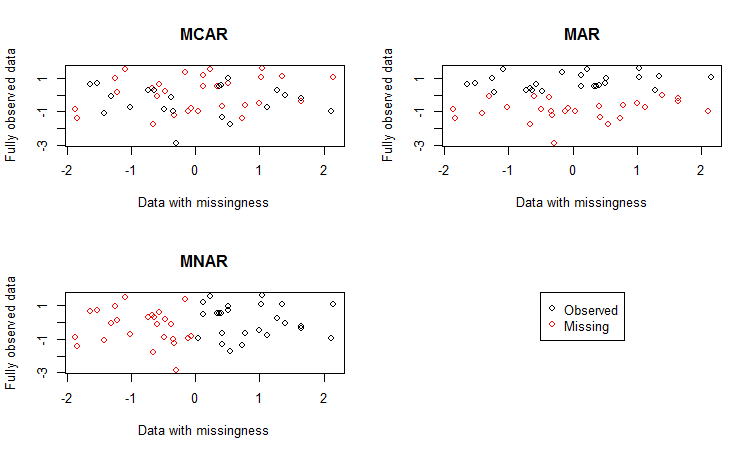
\includegraphics[width=0.95\textwidth]{md_mechanism}
  \caption{Visualization of Missing Data Mechanisms}
\medskip
Red dots indicate missing values, and black dots denote observed values. In each plot, the X axis is a covariate with missingness, and the Y axis is a fully observed covariate.
\label{fig:miviz}
\end{figure}


